\normallinespacing

\chapter{State of The Art}
\section{Education and technology}
This section introduces the main educational concepts and approaches used by teachers in this project. Among them, the incremental integration of technology with the classroom, and its challenges to researchers and teachers is a common thread.
\subsection{Computer-Supported Collaborative Learning (CSCL)}
Collaborative learning can take many forms depending on the teacher's approach, the pedagogical goal and the environment. At its core, CSCL is an approach to learning and sharing knowledge that stimulates the social nature of learning using diverse technological and pedagogical strategies \cite{Dillenbourg2009-jl}. As the name indicates, it relies on collaboration through technology to construct knowledge and solve problems. Group work is encouraged as it help students to engage with the learning materials \cite{Bonwell1991-sl}. The reliance on computers provides a wide range of tools and configurations that aid the teacher in working with this paradigm. Currently, collaborative learning is used all over the world and across all age levels of formal schooling \cite{Jeong2019-ul}.
\subsection{Scripts and Flow Patterns}
In CSCL, scripts define and manage learning objectives, types of activities, its sequencing and role distribution between students \cite{Kollar2006-lk}. Micro-scripts aim at triggering specific types of interactions that will generate learning gains. \cite{Dillenbourg2013-kx}. Macro-scripts \cite{Dillenbourg2008-kt} include individual activities and class-wide activities in addition to small group activities. A script will define a set of interactions in a learning activity and condition how the students will discuss and exchange opinions towards solving a problem.\\
Collaborative Learning Flow Patterns (CLFP) are examples of structures for macro scripts and refer to broadly accepted expert practices. They capture the structure of well-known collaboration scripts that can potentially lead to effective interactions \cite{Hernandez-leo2006-lv}. Pyramid is a type of CLFP that has been recognised as a good strategy for structuring CSCL activities \cite{Davis_undated-sg} and can be modified for students to collaborate and participate on numerous educational scenarios \cite{Hernandez-leo2006-lv}.\\
A Pyramid flow starts by dividing the class by a number, so that initial groups are formed. This number is defined by the teacher and is dependant on the length and the number of levels the activity should take to complete. This division creates an initial set of groups (at this point they might be as small as one student per group) each of which will solve a task. This task is common to all students in the class. Once every individual proposed a solution, the activity moves to the next level, in which groups are merged creating larger groups (by merging small groups), and the new ones (composed by individual groups from the previous level) have to agree on a common proposal. In next levels groups are merged again, repeating the same process: each new group has to discuss internally to reach an agreement on a proposal. This cycle repeats until a consensus is reached at a global level. This way, Pyramid fosters individual participation and accountability \cite{Hernandez-leo2006-lv}. Most importantly, Pyramid can be applied to a wide range of problems and topics, which makes it a versatile flow. Figure 1 is a representation of this flow.
\begin{figure}[!h]
    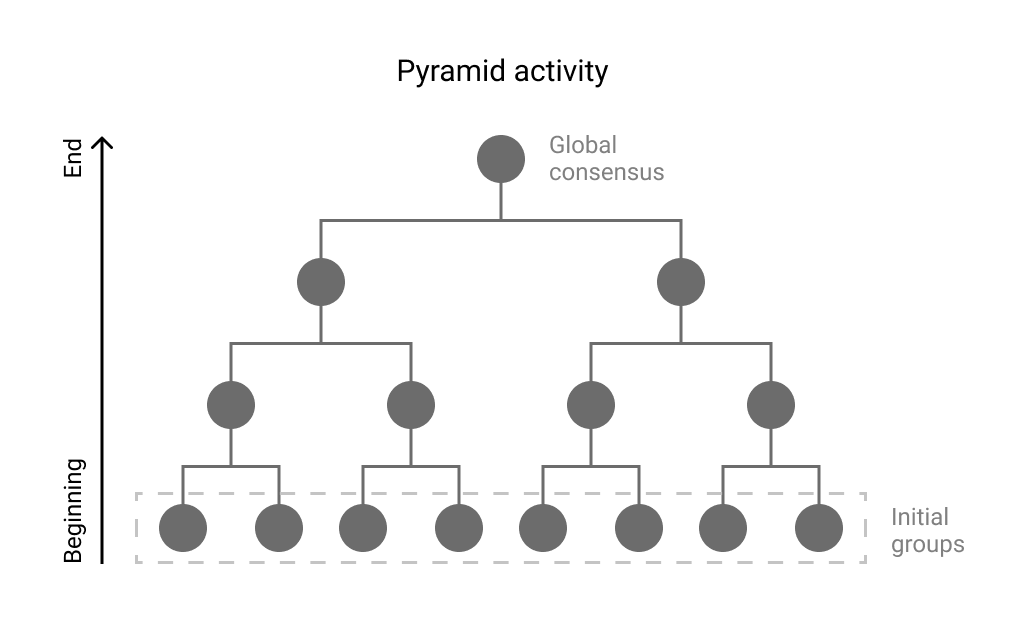
\includegraphics[clip,width=\columnwidth]{Figures/pyramid-activity.png}% 
\caption{Diagram of pyramid activity}
\label{fig:pyramid}
\end{figure}
This particular type of flow pattern (and a tool that supports it) will be used by teachers in the measurements for this project.
\subsection{Research in CSCL}
Research in CSCL has been growing since 1990 \cite{Dillenbourg2009-jl}. After going through periods of building a shared, initial understanding of the knowledge, and a notable growth in the scientific community \cite{Dillenbourg2009-jl} it is currently facing the challenges of integration with the fast-paced evolution of technology. These challenges include ensuring the accumulation of CSCL research knowledge in the face of the wide heterogeneity of concepts and methods, and the research of a dynamic that naturally presents a multiplicity of interacting factors.\\
Computer software is a resource for teachers to provide guidance, stimulate participation from students and for students to share knowledge. With the rapid growth and adoption of digital technology, experiments, tools, concepts and theories have expanded as well \cite{Dillenbourg2009-jl}. As the scientific community directs efforts towards understanding the most effective way to introduce technology in the classroom (or adapt current technology) it becomes apparent that the success of CSCL tools is hidden in the implementation details \cite{Dillenbourg2011-zr}. This includes having a deep understanding of particular environments for different teachers, defining amount of information being displayed on  each tool, and designing the appropriate user interface, as users could get overwhelmed by the amount of information presented to them. \cite{Schwendimann2017-ci}\\
Not only implementation details are key to have a positive and lasting impact in the teaching experience, but the standardisation of measurements and evaluations of tools and practices becomes increasingly necessary as well to build a body of knowledge in the scientific community.
\subsection{Learning Design, Learning Analytics and Teacher-facing dashboards}
Research on instructional and learning design (LD) focuses on complex learning environments, and access to the learner data available in these environments \cite{Wasson2020-lq}. The advent of technology has moved the focus from learning content and how it is sequenced to learning environments as a whole. This means that there is a move from traditional instructional design and tools to support teachers, to a wider understanding of the interactions, tools and frameworks that aggregate in a learning environment.\\
This growing field of study focuses in supporting teachers as designers \cite{Kirschner2015-yg}, as they are increasingly required to have knowledge and skills to integrate digital technology into their classroom. For a teacher to create a fruitful learning environment, it is critical that they are aware and skilled in different techniques, tools, and ingredients (content domain, cues, 360-degree feedback, etc.). Furthermore, the ability to decide which tool to use, when and in which situations is also a skill that needs to be developed to create successful teacher-learner dynamics.\\
Researchers and practitioners in the field of LD are increasingly focusing in the integration of Learning Analytics (LA) as a tool to make pedagogical decisions to improve a learning environment. LA is the analysis and representation of data about learners in order to improve learning \cite{Siemens2012-nf}. For this analysis, data about learners experiences and programs is measured, collected and reported \cite{Clow2013-ww}.
In the context of Learning Analytics, dashboards are defined as a single display that aggregates multiple visualisations of different indicators about learner(s), learning process(es) and/or learning context(s) \cite{Schwendimann2017-ci} As students engage in CSCL activities, information about their activity and performance can be presented to the teacher through a dashboard. Teachers can use this information to assess the progress of the activity to make pedagogical decisions for the class and to plan interactions with individual students \cite{Xhakaj_undated-xx}.\\
Even though the development and analysis of teacher-facing dashboards is growing, there is little agreement on the best practices to design one. \cite{Schwendimann2017-ci} There is a lack of comparative studies among different dashboards (a type of teacher-facing visualization) or dashboard design options (in part due to the difficulty in achieving controlled yet relatively authentic conditions, but also due to a lack of widely-accepted, specific evaluative constructs, beyond general ones like usability or usefulness). \\
By capturing, analysing and visualising data traces that represent students’ collaborative interactions in real-time, LA offers the possibility for teachers to obtain a deeper understanding of the process of collaboration and student activity engagement \cite{Jivet2018-nw}. 
\section{Orchestration Load Measurements}
This section introduces concepts that allow us to operationalise how teachers manage a class in real-time. Also, approaches for measurement are discussed.
\subsection{Definitions}
In the setting of a class, a teacher not only manages the core activities (designed by themselves for the class), but also keeps track of timing, student performance, and manages extraneous events \cite{Dillenbourg2013-kx}. \\
In the field of Technology-Enhanced Learning, orchestration refers to “how a teacher manages, in real-time multi-layered activities in a multi-constraint context” \cite{Dillenbourg2013-kx}. A CSCL activity requires the teacher to monitor the students' activity and performance to provide guidance and make pedagogical decisions in the moment, and a dashboard delivering pertinent information in real time will help teachers in making those decisions. However, "the number of studies that investigate whether the addition of teacher-facing dashboard applications influence orchestration load of the teacher is scarce." \cite{Amarasinghe2020-wt}. If there is lack of fit between the technological environment's demand and the technological abilities of the teacher, or a lack of technical support from the institution, the teacher may experience increased levels of stress \cite{Al-Fudail2008-zo}.\\
Currently, orchestration load is still a fuzzy and an abstract concept, \cite{Prieto2015-gd} but we can safely assume that it has a cognitive component to it (remembering the content to be explained, modelling students’ learning progress, deciding how to adapt the lesson plan).
\subsection{Measurements}
Cognitive load, is the mental effort needed by a human to perform a certain task \cite{Wang2005-nv}. It has been extensively used in human-computer interaction and usability researchers have devised multiple direct and indirect methods to measure it. To assess orchestration load, It would be possible to draw from the methods developed to measure cognitive load. The difference between both is that the latter is usually measured in controlled lab environments, while orchestration load takes place in a class with students, which presents a multiplicity of variables that are virtually impossible to control. Introducing an activity to measure cognitive load (e.g., a dual task activity) to the subject is possible in a lab environment, but quite challenging if a teacher has to do it while managing a class in real time. Consequently, this only leaves us with indirect measures of orchestration load based which track involuntarily physical reactions of the subject, (e.g., variations in temperature, and pupillary dilation) and subjective measures (e.g., questionnaires) \cite{Prieto2018-vw}.\\
Electrodermal Activity (EDA) is an electrical phenomenon involving the sweat glands that occurs because of excitement or strain. It is observed as changes in the resistance of the skin to a small electrical current, or as differences in the electrical potential between different parts of the skin. It is used as an index to measure affective degree such as stress, strain, and excitement in psychology \cite{Kurniawan2013-ti}.\\
Even though it is proved that EDA varies with excitement or stress, a study on teacher stress when using technology found that at times EDA variances were observed at times where a teacher reported no stress \cite{Nepal_Ojashwi_and_Rk_Jha_and_Bk_Kapoor_undated-ni}. Also there were no EDA variances in situations where the subject reported being stressed \cite{Al-Fudail2008-zo}. This reveals that involuntary physical reactions like EDA should not be the only measurement taken to assess orchestration load. 
Prieto et al proposed a mixed-method approach to the measurement of orchestration load \cite{Prieto2015-gd} that gathers qualitative and quantitative data from indirect measures (EDA) and self-perception measures (Questionnaires). Gathered data is then triangulated to understand how the orchestration process takes place. This approach allows to have a multi-perspective view of the orchestration load a teacher experiences during a particular context.\\
This project aims to look for the correlation of orchestration load of a teacher using PyramidApp with different aspects of the interface. To do this, the orchestration load of teachers will be observed from different perspectives in a mixed-method approach.
\section{Usability Evaluations and Field Research}
The interface's easiness of use (usability) needs to be operationalized so that we can know how variations in orchestration load are related to it. This section introduces the basic concepts needed to operationalize usability, and introduces methods for measurement.
\subsection{Definitions}
The ISO 9241-11 standard defines usability as the capability of a product to be used by certain users to achieve specific objectives with effectiveness, efficiency, and satisfaction within a specific use context \cite{noauthor_undated-ex}. Usability is an important consideration in the design of products because it is concerned with the extent to which the users of products are able to work effectively, efficiently and with satisfaction. If a class is working using CSCL practices, the presence of digital products is necessary for the main activities in the classroom to take place. A tool that doesn't simplify tasks could add to the workload a teacher already has. Thus, usability of the selected software becomes of critical importance. Though this concept (a quality of all objects we use) is inherently subjective, it can be measured and evaluated using a variety of methods.
\subsection{Evaluation Methods}
An usability evaluation method is a procedure composed by a set of activities for collecting data of users interacting with a software. \cite{Fernandez2011-ln}. As internet became part of our lives, the challenge of developing more user-friendly interfaces led to the emergence of methods, techniques and tools through which usability can be assessed.
Usability evaluation frameworks are under development since 1971 \cite{Scholtz_undated-ip}. Each framework uses a particular methodology, and adapts itself to different resources, research goals, and technological environments, giving HCI specialists a broad range of options to pick from when analysing an interface. Some of these frameworks include usability testing, heuristic evaluations, rapid prototyping and cognitive walkthroughs.
\subsection{Types of evaluations}
In his research, Scholtz \cite{Scholtz_undated-ip} describes some usability evaluation methods (UEMs). He mentions user-centered and expert-based as the most recurrent methods to assess an interface.\\
In user-centered methods representative users are recruited for them to interact with the interface to be assessed. The user is recorded completing tasks previously defined by the researcher, and data from the recordings is later processed to detect usability problems. The main advantage of these methods is the involvement of users. Results and conclusions of user-centered methods are based on what happened to representative users during the tests. Downsides of this approach include the operative cost of recruiting representative users and the need for a sufficiently developed interface for testing. Usually, users are invited to go to a laboratory or office where the tests will take place, which can interfere with the authenticity of the real context of usage, since the user wouldn't be testing the software in a familiar environment. \\
Expert-based methods are performed by HCI experts by analysing usability aspects of the software and its compliance to a given set of guidelines. Analysts use already-established usability guidelines, or a set of guidelines specific for a particular product (e.g., an Android app can be analysed using Google's Material Design guidelines to ensure coherence with the operative system). Through this analysis, an expert is able to detect problems and inconsistencies in an interface. Heuristic evaluation is the most adopted type of expert-based inspection method and a well known set of usability heuristics was developed by Jakob Nielsen in 1994 (Table 1). It is continuously updated to this day.
{\footnotesize
\begin{table}
    \caption{Ten Usability Heuristics}
    \vspace{5mm}
    \begin{tabular}{ |p{4cm}|p{10.1cm}| }
        \hline
        1. Visibility of system status&The design should always keep users informed about what is going on, through appropriate feedback within a reasonable amount of time.\\
        \hline
        2. Match between system and the real world&The design should speak the users' language. Use words, phrases, and concepts familiar to the user, rather than internal jargon. Follow real-world conventions, making information appear in a natural and logical order.\\
        \hline
        3. User control and freedom&Users often perform actions by mistake. They need a clearly marked "emergency exit" to leave the unwanted action without having to go through an extended process.\\
        \hline
        4. Consistency and standards&Users should not have to wonder whether different words, situations, or actions mean the same thing. Follow platform and industry conventions.\\
        \hline
        5. Error prevention&Good error messages are important, but the best designs carefully prevent problems from occurring in the first place. Either eliminate error-prone conditions, or check for them and present users with a confirmation option before they commit to the action.\\
        \hline
        6. Recognition rather than recall&Minimize the user's memory load by making elements, actions, and options visible. The user should not have to remember information from one part of the interface to another. Information required to use the design (e.g., field labels or menu items) should be visible or easily retrievable when needed.\\
        \hline
        7. Flexibility and efficiency of use&Shortcuts — hidden from novice users — may speed up the interaction for the expert user such that the design can cater to both inexperienced and experienced users. Allow users to tailor frequent actions.\\
        \hline
        8. Aesthetic and minimalist design&Interfaces should not contain information which is irrelevant or rarely needed. Every extra unit of information in an interface competes with the relevant units of information and diminishes their relative visibility.\\
        \hline
        9. Help users recognize, diagnose, and recover from errors&Error messages should be expressed in plain language (no error codes), precisely indicate the problem, and constructively suggest a solution.\\
        \hline
        10. Help and documentation&It’s best if the system doesn’t need any additional explanation. However, it may be necessary to provide documentation to help users understand how to complete their tasks.\\
        \hline
    \end{tabular}
    \cite{heuristics}
\end{table}
}\\
When using this method, it is recommended to aggregate findings from different evaluators, since each evaluator is likely to detect different usability problems. Nielsen \cite{Nielsen1994-un} recommends to involve between three and five evaluators. In a study, he analysed the findings from multiple evaluators, looking to understand the payoff of using multiple evaluators. Figure 2 shows the proportion of usability issues detected by evaluators.
\begin{figure}[!h]
    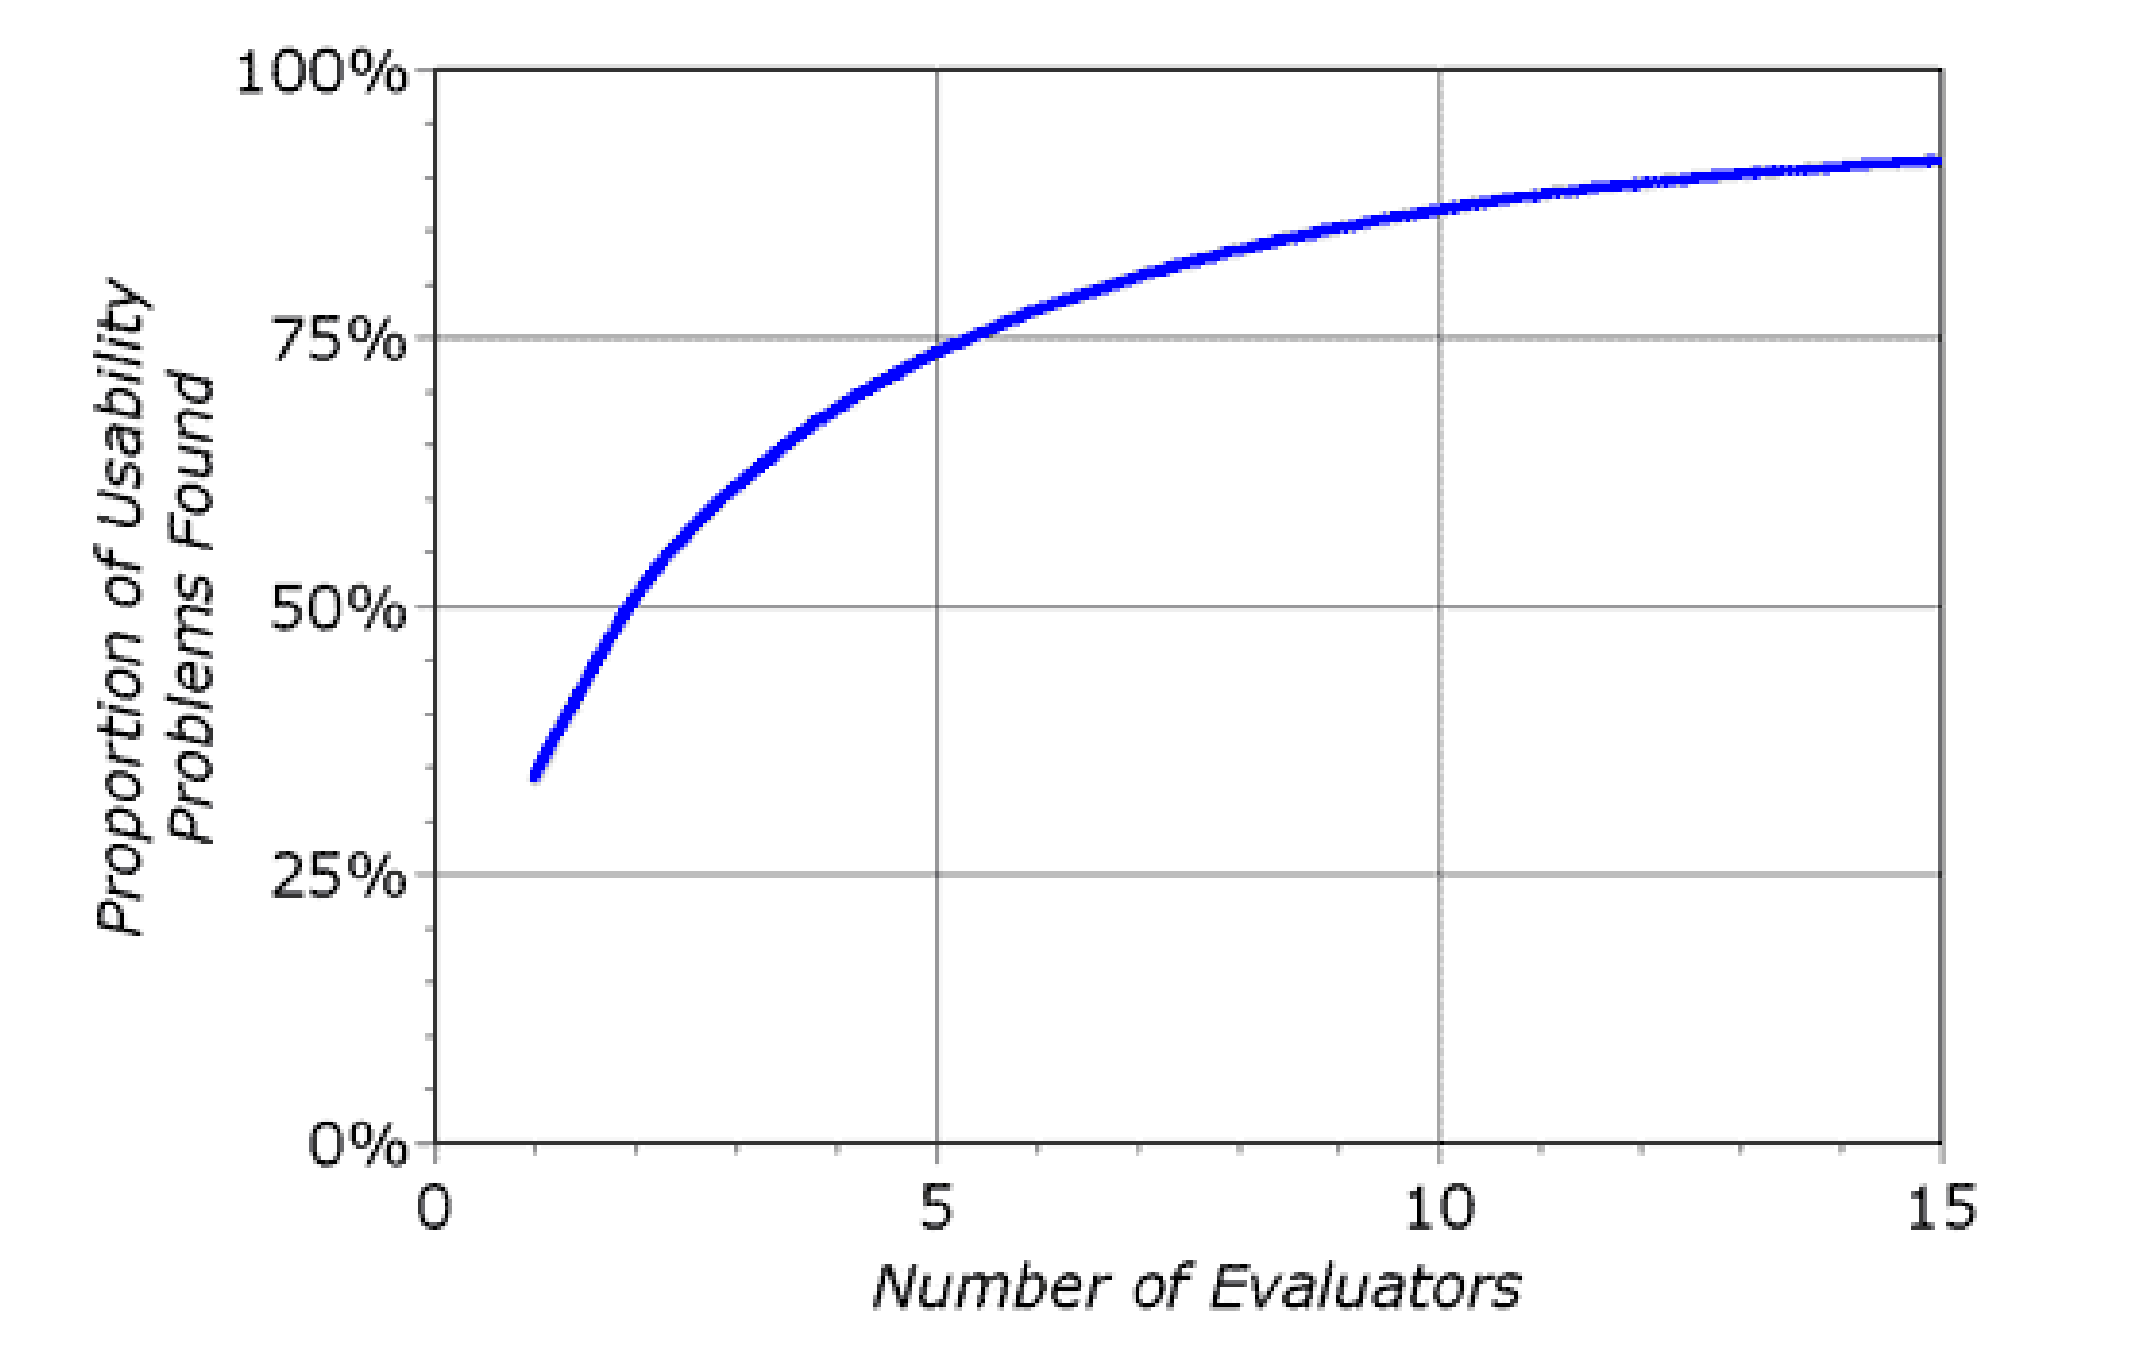
\includegraphics[clip,width=\columnwidth]{Figures/evaluators.png}% 
\caption{Diagram of pyramid activity}
\label{fig:timeseries}
\cite{Nielsen_undated-po}
\end{figure}\\
Expert-based methods usually imply less operative costs (they can be done by a single person) and are more versatile to the stage of development (they can be done at early and implementation stages similarly).  However, they do not provide possible solutions the usability issues they might  detect. Moreover, it might be difficult to draw conclusions from multiple evaluators as the report problems at different levels.\\
Gray and Salzman \cite{Gray1998-oo} conducted an analysis of five experiments that compared UEMs. The aim of their study was to demonstrate that there is a definite need for scientific rigor in experiments of this type. The researchers concluded with a set of recommendations for researchers using HCI evaluation methods in scientific experiments. According to the authors, since there is no easy way of knowing truth, researchers should seek convergence of measurements from multiple performance measures. These measurements need to be carefully analysed before concluding that they are related to a particular usability problem. Based on this recommendation, we will combine an expert-based usability evaluation with recordings of the subjects of this experiment. Both recordings of the users in their environment and of their screen while using the app will be analysed. Definitions and procedures of this methodology are described in the following section.
\subsection{Field research}
Field Research is a general method for collecting data that relies on an observational approach involving a relationship between the researcher and the subject of the research \cite{Burgess2003-oy}. This type of research has been principally conducted by social anthropologists and sociologists and is known as fieldwork, ethnography, case study, qualitative research, interpretative procedures and field research.  Participant observation, interviews and documentary evidence are some of the resources field researchers use to elucidate the meaning of the subject's behaviour \cite{Burgess2003-oy}.\\
Alongside observational work, formal and informal interviews may be conducted and life histories and personal documents may be collected. In addition, techniques will need to be developed for gathering, storing, retrieving and analysing data as well as checking the reliability and validity of that data.\\
In his book, Burgess \cite{Burgess2003-oy} argues that Field Research is a term with diverse connotations and slight differences for each science it is used for. This is why it is generally defined as a method for collecting data. Schatzman and Strauss assert that "The field researcher is a methodological pragmatist. He sees any method of inquiry as a system of strategies and operations designed -at any time— for getting answers to certain questions about events which interest him." \cite{Schatzman1972-zz}\\
Field research is being increasingly used in HCI (\cite{Millen_undated-et}; \cite{Pensabe-Rodriguez2020-qs}), as observing users can provide meaningful insights about their behaviour and needs. This information can be helpful when developing or analysing a digital product. Digital cameras and screen-recording software enables researchers to analyse subjects' behaviour while they operate in their familiar environment (i.e., their offices) in an unobtrusive manner, to analyse in a later stage.\\
The importance of ethnographic research in design has been described by Blomberg \cite{Schuler2017-ka}. These methods provide the developers with a richer understanding of the context of the users when interacting with an interface. Observing representative users in their environment might shine a light on user requirements that would be hard for users to articulate.
\section {Mixed methods for this project}
For this project, representative users are be teachers who are already integrating CSCL practices into their teaching and that would be interested in using PyramidApp in their classes. Furthermore, they would need to be located near the researchers, since measurements for this experiments will be done in person. We estimate that sourcing for representative users with this conditions would imply costs that are out of reach for the context of this project. For these reasons, user-centered methodologies will not be applied. Instead, the usability of PyramidApp will be assessed using a combination of expert-based methodologies and recordings from field research.
\section{Closing remarks on the state of the art}
This section has presented the main concepts methodologies that will be part of the experimental setup of the project. By triangulating information of the subjects' EDA, self-perception measures and usability assessments we will be able to elucidate the relationship of orchestration load and usability factors in PyramidApp.

%\section{Objectives}
%\section{Structure of the Report}


\newpage


